\documentclass[11pt]{article}
\usepackage[final]{acl}
\usepackage{times}
\usepackage{latexsym}
\usepackage[T1]{fontenc}
\usepackage[utf8]{inputenc}
\usepackage{microtype}
\usepackage{inconsolata}
\usepackage{graphicx}
\usepackage{booktabs}
\usepackage{array}
\usepackage{tabularx}
\usepackage{amsmath}
\usepackage{placeins}
\usepackage{float}
\usepackage{tikz}
\usetikzlibrary{positioning,arrows.meta}

\usepackage{hyperref}

\newcommand{\method}[1]{\textbf{M#1}}
\newcommand{\nr}{\mathrm{NR}}

\title{What Is the Price of a Model's Eye?\\
Understanding How VLMs Answer Multiple-Choice Questions in Multimodal Settings\\
Final Report}
\author{Divyanshu Giri, Rachit Mehta, Yashav Bhatnagar \\
        IIIT Hyderabad}

\begin{document}
\maketitle

\begin{abstract}
MCQA is a key competence of vision-language
models that is tested by a variety of mainstream
benchmarks. However, these models can have
a wide range of changes in performance when
the task is diversified even slightly. The question we are asking is: how do mainstream
vision-language models perform on formatted multiple-choice question answering tasks?
Using a counterfactual dataset derived from
CLEVR scenes, we set out to evaluate and understand the models’ internal representations
by employing methods like layer-wise activation patching, individual attention head localization, and vocabulary projection for answer
choices to localize key hidden states and activation patterns that encode information about
predictive tokens. Our experiments suggest that visual information is available early in
image tokens, passes through option-content semantic representations in the middle layers, and
reach the answer position and symbols in the
late layers, mainly through attention. We find
that all answer labels show a late increase in the
logits, while a sparse set of attention heads separates the correct label. We also observe that
common answer alphabets are more robustly
promoted in vocabulary space than rare symbols. Our work  extends this analysis to other model families and to vision specific experiments separating visual-grounding
features from symbol-binding features.\footnote{Code is available at \url{https://github.com/DivyG007/vlm-mcqa}}
\end{abstract}

\section{Introduction}

Multiple-choice question answering (MCQA) is widely used to evaluate language models \citep{wiegreffe2025answerassembleaceunderstanding} and vision-language models \citep{meng2024mmiumultimodalmultiimageunderstanding}. MMMU \citep{yue2024mmmu} and its successor \citep{yue2025mmmuprorobustmultidisciplinemultimodal} evaluate multimodal models across many disciplines. The successor removes questions that text-only models can answer, expands the answer choices and adds a vision-only setting, under which VLM performance drops significantly. At the same time, text-only models are sensitive to seemingly minor changes such as moving the correct answer or changing its label \citep{pezeshkpour2024large,alzahrani2024when,khatun2024study,zheng2024large}. These observations motivate looking inside the model to understand how an answer is formed.

Our focus is on which internal states and attention heads produce the answer. A VLM can understand the image yet emit the wrong symbol, or be steered by a symbol without the matching content. We therefore separate three quantities: the \emph{visual answer content} (the image and question imply ``brown''), the \emph{option position} (``brown'' is the first displayed option), and the \emph{output symbol} (that option is labelled A). Relabelling the first option Q changes the required symbol while leaving its position and content unchanged. Building on the text-only analysis of \citet{wiegreffe2025answerassembleaceunderstanding}, we ask where and through which components VLMs connect these quantities.

We use controlled CLEVR image pairs and independently vary the visual answer, option order and label alphabet. We conduct seven experiments combining activation patching with Logit Lens and Tuned Lens analysis. Activation patching tests which internal states and attention heads causally affect the answer; the lenses track when answer content, output labels and the requested alphabet become readable through the model's layers.

Our contributions are:
\begin{enumerate}
\item A seven-experiment comparison across Qwen, InternVL, LLaVA and PaliGemma2, with a transfer test on controlled IconQA image pairs.
\item A trained Tuned Lens for each model, testing whether information is readable earlier than an untrained vocabulary readout suggests.
\item Four vision-specific studies of image restoration, wrong-answer repair, spatial attention and picture answer options.
\end{enumerate}

\section{Related Work}
\label{sec:related-work}

Option order and output symbols can alter MCQA predictions despite unchanged alternatives \citep{zheng2024large}; \citet{atabuzzaman2025benchmarking} and \citet{zeno2025choosing} report token, position and selection biases in visual MCQA, motivating a search for the components that connect visual answer content to the emitted label.

In Answer, Assemble, Ace (AAA), \citet{wiegreffe2025answerassembleaceunderstanding} combine vocabulary projections and activation patching under option-position and alphabet changes to distinguish answer representations from output-symbol promotion in text-only MCQA. \citet{wong2026decidebind} use trained probes and probe-aligned interventions, finding answer-relevant information at option boundaries and stronger symbol-binding effects near the output. Correct-letter head analyses localize answer-label contributions, while path patching of symbol-biased heads localizes sensitivity to output alphabets \citep{lieberum2023doescircuit,yang2025option}. Readout accessibility alone does not establish where answer information is first computed or causally used \citep{wiegreffe2025answerassembleaceunderstanding,wong2026decidebind}. Patching outcomes depend on corruption and metrics, and component selection can amplify instability \citep{zhang2024patching,heimersheim2024patching,meloux2026statistical}. The logit lens reads intermediate states through the output unembedding \citep{nostalgebraist2020logitlens}; the Tuned Lens instead learns one affine translator per layer and gives more faithful intermediate predictions \citep{belrose2023tunedlens}.

In VLMs, activation swaps with downstream context cached can redirect object--word associations \citep{saravanan2025binding}, while controlled swaps and head interventions provide evidence for spatial indexing and feature retrieval \citep{assouel2026visualsymbolic}. \citet{golovanevsky2025notice} introduce NOTICE, separating semantic image-pair corruption from candidate-word replacement and patching multimodal modules and heads. \citet{palacios2026abstraction} report intermediate semantic separation before late vocabulary-letter alignment in VLMs. We adapt AAA's answer-to-label analysis and NOTICE's semantic image interventions to controlled visual MCQA, and add frozen-head mediation, error repair, spatial-edge blocking and visual-option tests that target the content-to-symbol step directly.

\section{Task, Data and Models}

\subsection{Datasets: CLEVR-MCQ-4 and IconQA}

Repeated activation patching needs many correctly answered, controlled donor and recipient pairs. On heterogeneous expert benchmarks such as MMMU \citep{yue2024mmmu}, a failed patch on a sub-10B model is hard to distinguish from basic incapacity. We therefore built CLEVR-MCQ-4 from CLEVR's diagnostic scenes and functional programs \citep{Johnson_2017_CVPR}: nine reasoning families (e.g.\ colour of a related object, counting, logical OR) with four type-matched options.

\paragraph{Counterfactual pairs and prompts.} Each pair contains an original CLEVR image and an edited image whose correct answer changes, with the question and answer alternatives fixed. We vary option order and three label alphabets to separate answer content, position and output symbol. The release contains 1,252 items, 17,328 prompt variants and 14,400 directed contrasts, partitioned into scene-disjoint splits. Appendix~\ref{app:example} gives an example and the full construction, prompt and split details.

\paragraph{Controlled IconQA subset.} To test transfer beyond synthetic renders we use one IconQA task \citep{lu2021iconqa}: native four-text-choice marble-probability questions (certain, probable, unlikely, impossible) from two grade families. No exact answer-changing native pairs exist, so each pair keeps the native image and replaces one marble's appearance at a fixed position and total count, which changes the answer; same-answer replacements are controls. The release has 8 calibration, 64 discovery and 64 confirmation source pairs with the same prompt format; causal methods use 32 correctly answered pairs per phase.

\begin{figure}[t]
\centering
\resizebox{\columnwidth}{!}{%
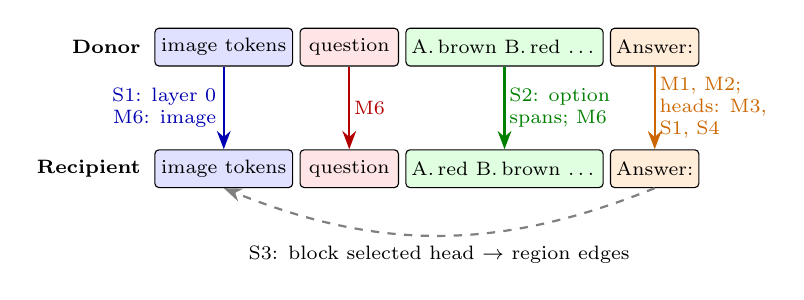
\begin{tikzpicture}[font=\scriptsize, >=Stealth,
  tok/.style={draw, rounded corners=1.5pt, minimum height=0.48cm, inner sep=2pt, align=center},
  arr/.style={->, thick}]
\node[tok, fill=blue!12, minimum width=1.75cm] (di) {image tokens};
\node[tok, fill=red!10, minimum width=1.25cm, right=0.08cm of di] (dq) {question};
\node[tok, fill=green!12, minimum width=2.15cm, right=0.08cm of dq] (do) {A.\,brown B.\,red \dots};
\node[tok, fill=orange!15, minimum width=1.0cm, right=0.08cm of do] (df) {Answer:};
\node[left=0.05cm of di, anchor=east] {\textbf{Donor}};
\node[tok, fill=blue!12, minimum width=1.75cm, below=1.05cm of di] (ri) {image tokens};
\node[tok, fill=red!10, minimum width=1.25cm, right=0.08cm of ri] (rq) {question};
\node[tok, fill=green!12, minimum width=2.15cm, right=0.08cm of rq] (ro) {A.\,red B.\,brown \dots};
\node[tok, fill=orange!15, minimum width=1.0cm, right=0.08cm of ro] (rf) {Answer:};
\node[left=0.05cm of ri, anchor=east] {\textbf{Recipient}};
\draw[arr, blue!70!black] (di) -- node[left, align=right, xshift=1pt] {S1: layer 0\\M6: image} (ri);
\draw[arr, red!70!black] (dq) -- node[right, xshift=-2pt] {M6} (rq);
\draw[arr, green!50!black] (do) -- node[right, align=left, xshift=-2pt] {S2: option\\spans; M6} (ro);
\draw[arr, orange!80!black] (df) -- node[right, align=left, xshift=-2pt] {M1, M2;\\heads: M3,\\S1, S4} (rf);
\draw[->, thick, dashed, gray] (rf.south) to[bend left=22] node[below, pos=0.5, text=black] {S3: block selected head $\rightarrow$ region edges} (ri.south);
\end{tikzpicture}}
\caption{Intervention sites. A patch copies one donor activation into the recipient at the same layer and token positions, or copies a donor head output into the same head at the recipient's final query position (``Answer:''). Everything else in the recipient run is unchanged. S4 uses the same sites with answer choices rendered as pictures.}
\label{fig:schematic}
\end{figure}

\subsection{Models}

We compare four open-weight VLMs (Table~\ref{tab:arch}). Qwen2.5-VL-7B, InternVL3.5-8B and LLaVA-OneVision-7B-SI use Qwen2.5-7B, Qwen3-8B and Qwen2-7B language backbones, respectively \citep{bai2025qwen25vl,wang2025internvl35,li2024llavaov}; PaliGemma2-10B uses Gemma2-9B \citep{beyer2024paligemma,steiner2024paligemma2}. On the vision side, ViT/InternViT and SigLIP encoders, together with different connectors, provide architectural variation. The twelve-checkpoint screening results are retained in Appendix~\ref{app:screen}.

\begin{table}[h]
\centering
\scriptsize
\setlength{\tabcolsep}{2pt}
\begin{tabularx}{\columnwidth}{@{}l>{\raggedright\arraybackslash}X>{\raggedright\arraybackslash}X>{\raggedright\arraybackslash}p{0.24\columnwidth}@{}}
\toprule
Model & Vision encoder & Connector & Language model \\
\midrule
Qwen2.5-VL-7B & native-resolution ViT, window attention & 2$\times$2 patch-merging MLP & Qwen2.5-7B, 28 L $\times$ 28 H \\
InternVL3.5-8B & InternViT-300M, 448-px tiles + thumbnail & pixel shuffle + MLP & Qwen3-8B, 36 L $\times$ 32 H \\
LLaVA-OV-7B-SI & SigLIP-So400m, any-resolution crops & 2-layer MLP & Qwen2-7B, 28 L $\times$ 28 H \\
PaliGemma2-10B & SigLIP-So400m, 448 px & linear & Gemma2-9B, 42 L \\
\bottomrule
\end{tabularx}
\caption{Architectures (L = decoder layers, H = attention heads per layer). All four place image tokens before the text prompt; PaliGemma2 attends fully over the image and prompt prefix.}
\label{tab:arch}
\end{table}

\subsection{Experimental setup and metrics}

\paragraph{Activation patching.} We run a donor prompt, cache one activation (a layer's residual state at chosen tokens, an attention or MLP update, or one head's output), rerun the recipient with that activation substituted, and measure how far the recipient's answer score moves toward the donor's. A residual patch replaces the whole hidden state, after attention and MLP have both written to it; a component patch replaces only one module's output at one layer.

\paragraph{Pair selection and evaluation.} Causal interventions use donor and recipient pairs that the model answers correctly: each model takes, in a fixed order, the first pairs of the shared scene pool that it answers correctly on both sides. \emph{Discovery} sweeps layers, heads and sites on the discovery split and fixes the chosen ones; \emph{confirmation} applies only those choices once to the scene-disjoint confirmation split.

\paragraph{Metrics and uncertainty.} For a predeclared logit difference $s$, normalized recovery is $\nr=(s_{\mathrm{patched}}-s_{\mathrm{recipient}})/(s_{\mathrm{donor}}-s_{\mathrm{recipient}})$: 0 means no movement and 1 means full donor transfer; it can exceed 1 and is not an accuracy. Accuracy is \emph{restricted four-label accuracy}: the largest logit among the four displayed labels. Confidence intervals are 95\% bootstrap intervals clustered at the independent unit (semantic pair or parent scene), not at prompt variants.



\section{Methods}

\subsection{Core-7}

Core-7 asks seven questions about how visual evidence becomes an answer symbol (Table~\ref{tab:core7}). M1, M2, M3 and M6 change internal activations; M4, M5 and M7 read those states without changing the model. Layers and heads are selected on discovery scenes and tested on separate confirmation scenes. Pair counts are provided in Appendix~\ref{app:extra}.

For M3, we average within each semantic pair before ranking heads, so every pair contributes equally. We select the top-$k$ heads ($k=1,2,4,8,16$) on discovery and keep those sets fixed for confirmation. Each is compared with 20 random sets containing the same number of heads in the same layers. Their 95th percentile is the score reached by only the best 5\% of random sets. A set is \emph{sparse} if four or fewer heads beat that baseline and recover at least 50\% of the effect of all heads in the selected layers.

\begin{table}[t]
\centering
\footnotesize
\begin{tabularx}{\columnwidth}{@{}l X@{}}
\toprule
 & Question and measurement \\
\midrule
\method{4} & When is the answer label readable? Project each residual stage to the vocabulary. \\
\method{5} & Is the content word readable before the label? Compare the two projections. \\
\method{7} & Do unfamiliar alphabets change the route? Repeat behaviour and readouts per alphabet. \\
\method{1} & When can a donor answer steer the output? Patch the final-token residual at every layer; unrelated pairs test contrast specificity. \\
\method{2} & Attention or MLP? Patch each layer's attention and MLP output at the final token, and replace each with another example's output. \\
\method{3} & Do a few heads dominate? Patch frozen top-$k$ head outputs in four discovery layers versus layer-matched random sets. \\
\method{6} & Which token groups carry the effect? Patch image, question, option-content or label tokens at every second layer. \\
\bottomrule
\end{tabularx}
\caption{Core-7. M1, M2, M3 and M6 intervene on activations; M4, M5 and M7 are observational readouts that measure vocabulary readability, not causal use.}
\label{tab:core7}
\end{table}

\subsection{Vision-specific extensions}
\label{sec:extensions}

Core-7 identifies useful states and heads, but leaves four questions about their visual role. The following studies use CLEVR-MCQ-4 scenes and each model's own four heads selected by Core-7, with 20 random four-head sets from the same layers as controls. Intervention sites are selected on discovery and tested on separate scenes.

\paragraph{S1: do the heads carry information from the image?} With the question and options fixed, we replace early image-token states with those from an answer-changing image. We then transfer the selected heads' outputs, or restore their original recipient values during image restoration, to measure how much of the image effect they carry.

\paragraph{S2: can option states repair a wrong answer symbol?} We select errors whose content readout favours the correct answer. We copy option-content states from a correctly answered prompt with reordered options, while keeping the recipient's labels. Success means recovering the recipient's correct symbol rather than copying the donor's.

\paragraph{S3: which image regions do the heads use?} We block the selected heads' attention to the object named by the question or to objects named by the options. Matched background regions control for the amount of attention removed.

\paragraph{S4: do the heads transfer meaning or copy a label?} We render the question and answer choices as pictures. The donor's correct object has a different label in the recipient, letting us distinguish transfer of the object from copying of the donor's symbol.

\subsection{Tuned Lens}

The Logit Lens applies the model's final output decoder directly to an intermediate hidden state. Earlier states may use a different representation, making information appear readable later than it is \citep{belrose2023tunedlens}. The Tuned Lens learns a small adjustment for each stage before applying the same decoder.

We train an affine translator $h \mapsto h + Ah + b$ at each residual stage, with $A$ and $b$ initially zero. The VLM stays fixed. A KL-divergence loss trains the decoded distribution to match the model's final output distribution. Training uses prompt text-token positions from separate screening and calibration scenes (360 training, 60 validation; 250 updates); images remain part of the model input.

Both lenses are evaluated on the same 3,072 behaviour variants. A readout milestone is the first stage where both the mean score and its 95\% confidence interval's lower bound exceed the threshold for that measurement.

\section{Results}

\subsection{Behaviour and image dependence}

All models use the image: accuracy falls to near chance (25\%) with blank or shuffled images (Table~\ref{tab:behaviour}). InternVL is most accurate and image-dependent; LLaVA formats perfectly but is less accurate, and PaliGemma2 solves only about half the items. Logical OR is the weakest family for Qwen and LLaVA (44.7\% and 31.6\%).

\begin{table}[t]
\centering
\footnotesize
\setlength{\tabcolsep}{3pt}
\begin{tabularx}{\columnwidth}{@{}X*{4}{c}@{}}
\toprule
 & Qwen & InternVL & LLaVA & Pali \\
\midrule
A/B/C/D & 83.7 & 91.2 & 65.3 & 54.4 \\
1/2/3/4 & 80.3 & 78.3 & 63.6 & 52.6 \\
Q/Z/R/X & 82.2 & 85.5 & 62.9 & 52.8 \\
Worst position & 81.3 & 90.2 & 60.6 & 48.8 \\
Blank image & 28.5 & 28.8 & 28.0 & 28.8 \\
Shuffled image & 29.6 & 29.3 & 26.9 & 28.0 \\
Clean$-$shuffled & 54.1 & 61.9 & 38.5 & 26.4 \\
\bottomrule
\end{tabularx}
\caption{Restricted four-label accuracy (\%) on the 256-item behaviour split, 1,024 variants per alphabet. Worst position is the lowest A/B/C/D accuracy over the four correct-answer positions. Pali: PaliGemma2.}
\label{tab:behaviour}
\end{table}


\subsection{M4, M5 and M7: readable content and output symbols}

\paragraph{Method.} At the final prompt token, the Logit Lens decodes each intermediate state into vocabulary scores. M4 tracks the correct label, M5 compares it with the answer word, and M7 varies the output alphabet.

\paragraph{Results.} With A/B/C/D, the correct label first becomes readable at stages 22, 25, 25 and 35 in Qwen, InternVL, LLaVA and PaliGemma2. A stage is the residual state entering that decoder layer. In the first three models, the content word becomes readable only at stage 27; in PaliGemma2 it remains unreadable even at the output (Appendix~\ref{app:tuned}). Thus the final token makes the label readable before the content word.

With rare letters, the Logit Lens shows little probability mass on the requested alphabet until late: Qwen rises from 0.13 at stage 24 to 0.83 at 25, and LLaVA from 0.01 to 0.72 at its late transition. This suggests an apparent late switch from default A/B/C/D labels to the requested alphabet.

\paragraph{Interpretation.} Late content-word readability at the final token does not mean visual content is absent earlier: The M6 interventions reported below locate it in image and option states. The alphabet-switch interpretation also depends on the readout, as the Tuned Lens comparison shows next.

\subsection{Tuned Lens: checking the readout}
\begin{figure}[t]
\centering
\includegraphics[width=\columnwidth]{figures/compact_lens.png}
\caption{Logit Lens (dashed) versus Tuned Lens (solid): (a) correct-label probability; (b) requested rare-alphabet share. Colours/markers identify models in both panels. PaliGemma2 is provisional.}
\label{fig:lens}
\end{figure}


\paragraph{Method.} We apply the trained stage-specific translators to the same hidden states and examples as the Logit Lens. We compare correct-label probability, content-word readability and probability mass on the requested alphabet.

\paragraph{Readout quality.} At the last translated stage, KL divergence from the model's final distribution falls from 7.64 to 0.050 in Qwen, 0.89 to 0.10 in InternVL, 1.10 to 0.027 in LLaVA and 2.06 to 0.16 in PaliGemma2.

\paragraph{The main label decision remains late.} Both lenses place the large jump in correct-label probability at the same stage, around 70--90\% of model depth (Figure~\ref{fig:lens}a). The Tuned Lens reveals weak earlier signals, including about 0.43 probability in LLaVA from stage 20 and 0.39 in InternVL from stage 22 with rare letters, against chance 0.25. The content word remains readable at the same stage as the label or later (Appendix~\ref{app:tuned}).

\paragraph{The requested alphabet is readable earlier.} In middle layers, the Tuned Lens reveals more mass on the requested rare alphabet than the Logit Lens (Figure~\ref{fig:lens}b). The alphabet is therefore readable before the final answer is decided, weakening the claim of a sudden last-layer alphabet switch. PaliGemma2's poorer middle-layer fit (KL about 0.76) keeps its Tuned Lens interpretation provisional.

\subsection{M1: when the final-token answer transfers}

\paragraph{Method.} We replace the final-token state with the donor's at each layer, under position, content and unrelated-pair contrasts.

\paragraph{Results.} Position transfer reaches normalized recovery 0.5 at layers 24, 29, 24 and 37 for Qwen, InternVL, LLaVA and PaliGemma2; content transfer crosses at 25, 31, 23 and 37 (Figure~\ref{fig:m1}). Position precedes content in Qwen and InternVL, content precedes position in LLaVA, and both cross together in PaliGemma2. The exact discovery-to-confirmation order is stable only in Qwen and InternVL (Table~\ref{tab:replication}).

\paragraph{Interpretation.} The final token develops a transferable answer state late. Unrelated donors also cross 0.5 at layers 24, 25, 24 and 39, so this state is not specific to counterfactual pairs.

\begin{figure}[t]
\centering
\includegraphics[width=\columnwidth]{figures/compact_m1.png}
\caption{M1: final-token transfer under position, content and unrelated-donor contrasts. Shading: 95\% intervals.}
\label{fig:m1}
\end{figure}

\subsection{M2: attention and MLP contributions}
\begin{figure}[t]
\centering
\includegraphics[width=\columnwidth]{figures/compact_m2.png}
\caption{M2: attention and MLP output patches at the final token. Attention carries the larger late effect in every model; shading gives 95\% intervals.}
\label{fig:components}
\end{figure}





\paragraph{Method.} We replace attention and MLP outputs separately at the final token. As a second check, we replace each component's output with that from an unrelated example and measure the drop in the correct answer's logit margin.

\paragraph{Results.} Attention-patch recovery exceeds MLP recovery in all four models (Figure~\ref{fig:components}). For Qwen, InternVL and LLaVA, attention peaks at layer 24 with recovery 0.44, 0.35 and 0.64, versus MLP peaks of 0.11, 0.05 and 0.10. PaliGemma2 peaks at layer 41 for attention (0.22) and layer 39 for the MLP (0.15).

Replacing layer-24 attention with an unrelated output lowers the correct answer's lead by 4.4, 5.6 and 5.0 logits in Qwen, InternVL and LLaVA; replacing the MLP at that layer lowers it by only 0.5, 0.1 and 0.6. In PaliGemma2, the corresponding drops at the peak layers are 2.3 logits for attention and 1.4 for the MLP.

\paragraph{Interpretation.} Late answer transfer is attention-dominated across all four models. PaliGemma2 has a larger relative MLP contribution, so the strength of this division varies across architectures.

\begin{table}[t]
\centering
\footnotesize
\setlength{\tabcolsep}{3pt}
\begin{tabularx}{\columnwidth}{@{}>{\raggedright\arraybackslash}X cccc@{}}
\toprule
Disc.\,/\,conf. & Qwen & InternVL & LLaVA & Pali \\
\midrule
Position-transfer layer & 24\,/\,24 & 29\,/\,29 & 24\,/\,24 & 37\,/\,37 \\
Content-transfer layer & 26\,/\,25 & 32\,/\,31 & 24\,/\,23 & 39\,/\,37 \\
Exact order replicates & yes & yes & \textbf{no} & \textbf{no} \\
Dominant component & attn & attn & attn & attn \\
Top-4 heads $\nr$ (conf.) & .417 & .441 & .580 & .618 \\
Random p95 (conf.) & .069 & .085 & .026 & .015 \\
Share of all-head effect & 52.7\% & 52.4\% & 71.3\% & 93.0\% \\
Sparse verdict & sp.\,/\,sp. & \textbf{dist.\,/\,sp.} & sp.\,/\,sp. & sp.\,/\,sp. \\
\bottomrule
\end{tabularx}
\caption{Core-7 comparison across all four models. Bold marks a change in ordering or sparsity verdict between discovery and confirmation. Pali denotes PaliGemma2; sp. and dist. mean sparse and distributed. All-head effect refers to the selected layers.}
\label{tab:replication}
\end{table}

\subsection{M3: important heads and model-dependent sparsity}
\begin{figure}[t]
\centering
\includegraphics[width=\columnwidth]{figures/compact_m3.png}
\caption{M3: selected top-$k$ heads (solid, 95\% intervals) versus layer-matched random-set 95th percentiles (dashed). The all-head reference covers the selected layers.}
\label{fig:m3}
\end{figure}


\paragraph{Method.} We rank individual heads on discovery, fix the top-$k$ sets, and evaluate their joint effect on confirmation. Random sets with the same number of heads in the same layers provide the baseline.




\paragraph{Results.} Four heads recover 0.417 [0.397, 0.438] in Qwen, 0.441 [0.405, 0.479] in InternVL, 0.580 [0.556, 0.602] in LLaVA and 0.618 [0.607, 0.630] in PaliGemma2 (Figure~\ref{fig:m3}). These are 52.7\%, 52.4\%, 71.3\% and 93.0\% of the effects of all heads in their selected layers, and all exceed the matched-random 95th percentile (Table~\ref{tab:replication}). PaliGemma2's top two heads already recover about 68\% of its all-head effect.

\paragraph{Interpretation.} A small selected head set carries a large answer-transfer effect in every model. The sparse verdict is stable in Qwen, LLaVA and PaliGemma2. InternVL crosses the 50\% boundary, from 49.9\% in discovery to 52.4\% in confirmation, so its categorical sparsity verdict is unstable. These results identify useful heads, without establishing a complete or uniquely necessary circuit.

\subsection{M6: which tokens carry the answer}

\paragraph{Method.} We replace image, question, option-content or label-token states separately, at every second layer under content contrasts.

\paragraph{Results.} Early image-token patches recover nearly the full donor effect in the three Qwen-lineage models; this decreases as question and option-content states become useful (Figure~\ref{fig:m6}). Option-content recovery peaks at 0.42 at layer 18 in Qwen, 0.24 at 22 in InternVL, 0.53 at 18 in LLaVA and 0.77 at 26 in PaliGemma2. PaliGemma2 also has a strong early image effect, with noisier later text-token effects. Label-token patches have little effect.

\paragraph{Interpretation.} Together with M1, the result supports useful image states early, option and question states in the middle, and an answer-symbol state late. These are useful sites, not an uninterrupted causal path.

\begin{figure}[t]
\centering
\includegraphics[width=\columnwidth]{figures/compact_m6.png}
\caption{M6: content recovery by token group. Image states dominate early; option and question states contribute later. Same confirmation cohorts as M1; shading gives 95\% intervals.}
\label{fig:m6}
\end{figure}

\subsection{S1: image restoration and head mediation}
\begin{figure}[t]
\centering
\includegraphics[width=\columnwidth]{figures/compact_s1_s2.png}
\caption{(a) S1: restoration, selected-head transfer and clamp (Qwen/InternVL: 24 held-out pairs), including LLaVA. S1 bars are point estimates. (b) S2: single-option discovery patches versus all-option confirmation at layer 20 (35 failures).}
\label{fig:restoration-repair}
\end{figure}


\paragraph{Method.} We keep the text fixed and test early image restoration, transfer through the selected heads, and the effect of resetting those heads during restoration.

\paragraph{Results.} Replacing all image-token states at layer 0 restores the donor effect almost completely on 24 held-out pairs (Figure~\ref{fig:restoration-repair}a): $+23.98$ logits [22.64, 25.16] in Qwen ($\nr$ 0.9998) and $+40.16$ [36.68, 43.99] in InternVL ($\nr$ 1.0002). Copying the four frozen head outputs transfers $+9.74$ logits in Qwen versus $+0.29$ for matched random heads, and $+17.72$ [16.09, 19.44] in InternVL, 17.82 [16.14, 19.59] above random; clamping the same heads during restoration removes almost exactly as much (9.74; 17.73).

\paragraph{Interpretation.} Across the three models, early image states carry most of the donor effect, and the selected heads carry a large, selective share. LLaVA shows the same pattern: image restoration gives +13.8 logits, selected-head transfer and clamp each give +7.8, and random heads remain near zero.



\subsection{S2: repairing a wrong final symbol}

\paragraph{Method.} We screen 3,072 saved behaviour variants each for Qwen and InternVL to select errors whose content readout favours the correct answer while the output symbol is wrong. We then test whether option-content patches recover the recipient's correct letter rather than the donor's.

\paragraph{Results.} In Qwen, single-option patches did not repair errors. Patching all four option-content spans at layer 20, while retaining the recipient's labels, raised the truth margin by 0.19 [0.11, 0.27] logits on 35 held-out failures and corrected 12.9\% [3.8\%, 24.3\%] (Figure~\ref{fig:restoration-repair}b); 2 of 72 matched correct cases were harmed. InternVL yielded no valid repair test. LLaVA's internal option readout aligned with the correct content in 71.6\% of selected scenes.

\paragraph{Interpretation.} Only the whole-option patch produced a modest repair in Qwen. This suggests that the relations among the options matter; a single correct-option state was insufficient.

\subsection{S3: spatial routing}
\begin{figure}[t]
\centering
\includegraphics[width=\columnwidth]{figures/compact_s3_s4.png}
\caption{(a) S3: harm beyond matched-background blocking (24 pairs); Qwen meets neither region criterion. (b) S4: heads-minus-random, content-minus-copy gain, and final content-minus-copy preference (Qwen/InternVL: 31 units), including LLaVA. Error bars: S3 only (95\%).}
\label{fig:spatial-copy}
\end{figure}


\paragraph{Method.} Discovery selected the image layer where erasing the named region hurt most relative to the control (Qwen 8, InternVL 5, LLaVA 4). A region counts as used only if, on held-out scenes, blocking it hurts more than blocking a background patch of the same number of image tokens, with the 95\% interval above zero.

\paragraph{Results.} Qwen met this criterion for neither region, with top-4 or top-16 heads (Appendix~\ref{app:extra}). InternVL's tiles and LLaVA's crops ruled out Qwen's shape-matched control, so theirs counts only tokens (a declared sensitivity). InternVL (layer 5, 24 pairs) uses the \emph{option} objects, 0.050 [0.018, 0.083] logits, not the question object, $-0.012$ [$-0.043$, 0.021]; LLaVA (layer 4, 24 pairs) uses the \emph{question} object, 0.052 [0.031, 0.076], not the option objects, $-0.015$ [$-0.025$, $-0.006$] (Figure~\ref{fig:spatial-copy}a).

\paragraph{Interpretation.} The supported region differs by model, and the effects are small. These tests do not establish one shared spatial routing pattern.

\subsection{S4: picture answer options}

\paragraph{Method.} Question and options are pictures labelled A--D; the donor's answer object sits under a different letter in the recipient, so moving there means content transfer and moving to the donor's letter means copying.

\paragraph{Results.} Patching one picture's early token states (query or answer option, layer 0 frozen in both models) favoured \emph{content} (Qwen discovery: +1.60 logits). The heads did the opposite (Figure~\ref{fig:spatial-copy}b). In Qwen (31 parents; a sensitivity without unrelated donors) they beat random heads by 0.75 [0.56, 0.93], yet the content letter gained less than the donor's letter, $-1.79$ [$-2.09$, $-1.51$], which still led by 2.05 [1.82, 2.28] logits after patching; InternVL (complete; 31 units) shows 2.15 [1.69, 2.67], $-4.49$ [$-5.11$, $-3.95$] and $-4.66$ [$-5.29$, $-4.01$].

\paragraph{Interpretation.} Early picture states transfer object content, but the selected heads favour the donor's letter. These results do not support clean content-to-recipient-symbol binding by those heads. LLaVA follows the letter-favouring pattern: +0.48 logits over random heads, $-0.76$ for content-minus-letter gain and $-0.72$ for final content-minus-letter preference.

\subsection{IconQA transfer}

\paragraph{Method.} We repeat the reduced Core-7 measurements on the controlled IconQA subset and test both newly selected heads and the heads selected on CLEVR.

\paragraph{Results.} The four models reproduce the broad late-attention and head-concentration findings (Table~\ref{tab:iconqa}). The first three models use the image (A/B/C/D accuracy 99.2, 95.1, 95.1\%; 35.2, 31.3, 27.3\% with a blank image); PaliGemma2 achieves 92.2\% accuracy. Label readability, the late alphabet jump, attention dominance and sparse new top-4 heads all recur. CLEVR heads transfer (3, 1, 4, 4 of 4 coincide with the new sets; InternVL's recover 49.6\%). With the text fixed, CLEVR heads patched from an answer-changing marble edit shift the margin 5.7, 14.0, 7.2 and 6.7 logits more than from a same-answer edit.

\paragraph{Interpretation.} The useful attention sites and selected heads transfer to this controlled probability task. Exact content/position ordering remains model-dependent; this single edited template does not establish transfer across IconQA as a whole.

\begin{table}[t]
\centering
\scriptsize
\setlength{\tabcolsep}{3pt}
\begin{tabularx}{\columnwidth}{@{}>{\raggedright\arraybackslash}X cccc@{}}
\toprule
IconQA confirmation & Qwen & InternVL & LLaVA & Pali \\
\midrule
M4 label readable (stage) & 21 & 25 & 20 & 29 \\
M5 content word readable & 28 & 34 & never & 34 \\
M7 rare-alphabet jump (stage) & 25 & 30 & 25 & 35 \\
M1 content\,/\,position layer & 23\,/\,24 & 24\,/\,30 & 19\,/\,24 & 27\,/\,39 \\
Exact order replicates & \textbf{no} & yes & yes & yes \\
M2 attention\,/\,MLP peak $\nr$ & .46\,/\,.15 & .25\,/\,.06 & .67\,/\,.08 & .24\,/\,.13 \\
M3 new top-4 $\nr$ (random p95) & .42 (.06) & .36 (.01) & .63 (.02) & .62 (.003) \\
Share: new\,/\,CLEVR top-4 & 53\,/\,53\% & 52\,/\,49.6\% & 74\,/\,74\% & 92\,/\,92\% \\
M6 image-group peak & L0 & L0 & L0 & L32 \\
\bottomrule
\end{tabularx}
\caption{IconQA reduced Core-7 (32 confirmation pairs per model). M4, M5 and M7 use the Logit Lens; M6 uses content-and-position contrasts. New top-4 heads are frozen on IconQA discovery; CLEVR top-4 are the frozen CLEVR Core-7 heads. Pali: PaliGemma2. Bold marks a non-replication.}
\label{tab:iconqa}
\end{table}



\FloatBarrier

\section{Conclusion}
\label{sec:conclusion}

Across four VLMs, causally useful sites follow one staged account: image tokens early, option and question tokens in the middle, and a few late attention heads that write the answer, also on IconQA. It stops at binding: repair is small, spatial routing is model-specific, and with picture options the heads carry the donor's letter, not its object.

\label{main-content-end}

\section*{Challenges and Limitations}
Core-7 sweeps took up to 34 hours for LLaVA on shared GPUs, limiting study coverage. LLaVA's option-state alignment does not establish a causal repair rate; PaliGemma2 S1--S4 were not run. IconQA required constructed counterfactual pairs rather than native answer-changing pairs.

Most causal evidence comes from synthetic scenes; IconQA covers one edited, class-imbalanced task template. Correct-only sampling favours easier examples. Three models share Qwen-lineage backbones. Useful patch sites do not establish a complete or minimal circuit. Lens readouts measure readability, and translators may benefit from more training. Modified-control studies support conclusions only for their stated designs.


\label{references-start}
\bibliography{references,v2_intro_references}

\clearpage
\appendix
\label{appendix-start}

\section{Example counterfactual pair}
\label{app:example}

\paragraph{Counterfactual pairs and prompts.} For a paired scene we find one edit (an object's colour, shape, size or material, or a swap of two objects for relation questions) that turns the answer into another displayed option, and re-render it. The pair is an original image $x$ and a counterfactual $y$ with identical question and options. Each item becomes 12 prompts: the options are rotated so the answer sits at each of the four positions, under three alphabets (A/B/C/D, 1/2/3/4 and rare letters Q/Z/R/X). A prompt is the question, four labelled options, ``Respond with only the option label.'' and ``Answer:''. Donor and recipient prompts form five contrasts: \emph{position} (same image, answer moved), \emph{content} ($x$ versus $y$ with the answer at the same position: same symbol, different content), \emph{content-and-position}, \emph{identity} (distractors permuted) and \emph{unrelated} pairs. The frozen release has 1,252 items, 17,328 prompt variants and 14,400 directed contrasts, split by scene before any analysis into calibration (120 items), screening (300), behaviour (256), discovery (320 items, 160 pairs) and confirmation (256 items, 128 pairs).


\begin{figure}[h]
\centering
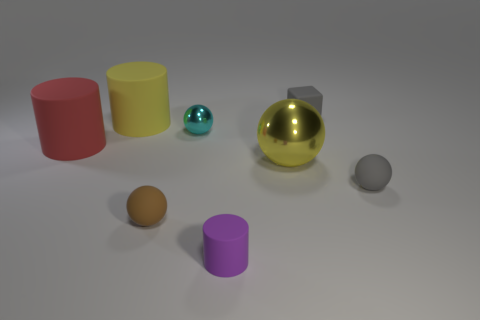
\includegraphics[width=0.49\columnwidth]{figures/example_pair_x.png}\hfill
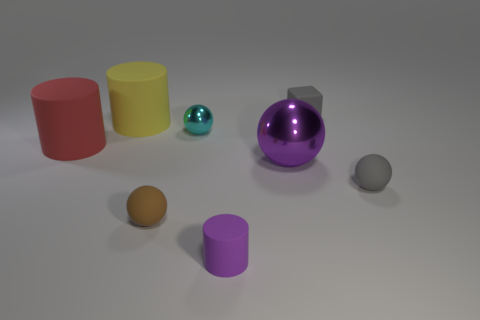
\includegraphics[width=0.49\columnwidth]{figures/example_pair_y.png}\\[2pt]
\scriptsize
\begin{minipage}[t]{0.49\columnwidth}\raggedright\ttfamily
What color is the large sphere that is in front of the yellow cylinder?\\
A. yellow\\ B. gray\\ C. red\\ D. purple\\
Respond with only the option label.\\
Answer:\quad\textrm{\textbf{A} (yellow)}
\end{minipage}\hfill
\begin{minipage}[t]{0.49\columnwidth}\raggedright\ttfamily
What color is the large sphere that is in front of the yellow cylinder?\\
A. purple\\ B. yellow\\ C. gray\\ D. red\\
Respond with only the option label.\\
Answer:\quad\textrm{\textbf{A} (purple)}
\end{minipage}
\caption{A confirmation pair (CLEVR scene 047521). Left: original image $x$; right: counterfactual $y$, re-rendered after one edit (the large sphere's colour, yellow$\to$purple). Both prompts put the answer at position A, so they form a \emph{content} contrast (same symbol, different content). The right-hand option order applied to image $x$ (answer B) forms a \emph{position} contrast with the left prompt. The numbers and rare-letter variants replace A--D with 1--4 or Q/Z/R/X.}
\label{fig:pair}
\end{figure}

\section{Model screening}
\label{app:screen}



\begin{table}[h]
\centering
\scriptsize
\setlength{\tabcolsep}{2.5pt}
\begin{tabular}{@{}llrrrr@{}}
\toprule
Family & Model (B) & Acc. & Worst pos. & Gap & D/C \\
\midrule
Qwen & Qwen2-VL (2.2) & .729 & .667 & .417 & 6/4 \\
Qwen & Qwen2.5-VL (3.8) & .844 & .833 & .573 & 6/6 \\
Qwen & \textbf{Qwen2.5-VL (8.3)} & .938 & .833 & .646 & 6/6 \\
InternVL & 3.5-1B (1.1) & .875 & .833 & .542 & 5/4 \\
InternVL & 3.5-2B (2.3) & .906 & .875 & .667 & 4/5 \\
InternVL & \textbf{3.5-8B (8.5)} & 1.000 & 1.000 & .781 & 6/5 \\
LLaVA-OV & 0.5B-SI (0.9) & .406 & .292 & .177 & 1/2 \\
LLaVA-OV & \textbf{7B-SI (8.0)} & .729 & .667 & .448 & 3/4 \\
LLaVA-OV & 7B-OV (8.0) & .646 & .625 & .354 & 6/6 \\
PaliGemma & 3B Mix (2.9) & .427 & .083 & .229 & 4/3 \\
PaliGemma & 2-3B Mix (3.0) & .500 & .125 & .260 & 2/3 \\
PaliGemma & \textbf{2-10B Mix (9.7)} & .583 & .542 & .396 & 2/3 \\
\bottomrule
\end{tabular}
\caption{24-item feasibility screen: restricted A/B/C/D accuracy, worst-position accuracy, clean-minus-shuffled gap, and usable discovery/confirmation pairs. Bold marks the family representative. Estimates use 24 items and are not pooled with later runs.}
\end{table}

\begin{table*}[t]
\centering
\scriptsize
\setlength{\tabcolsep}{2.5pt}
\begin{tabularx}{\textwidth}{@{}l>{\raggedright\arraybackslash}p{0.15\textwidth}>{\raggedright\arraybackslash}p{0.17\textwidth}>{\raggedright\arraybackslash}p{0.2\textwidth}>{\raggedright\arraybackslash}X>{\raggedright\arraybackslash}p{0.15\textwidth}@{}}
\toprule
Exp. & Question & What is patched & Layers / heads (Qwen; InternVL; LLaVA) & Main held-out result & What we learnt \\
\midrule
M1 & When can a donor answer steer the output? & Final-token residual state & Every layer & Position transfer crosses 0.5 at L24; L29; L24; unrelated donors cross at L24; L25; L24 & Late layers encode a transferable answer symbol, not pair-specific \\
M2 & Attention or MLP? & Attention or MLP output at the final token; patch, and replace with another example's & Every layer & Attention peaks at L24 (.44; .35; .64) vs MLP $\le$.11; L24 ablation 4.4; 5.6; 5.0 vs 0.5; 0.1; 0.6 logits & Late transfer is attention-dominated \\
M3 & Do a few heads dominate? & Head outputs at the final query & Layers 19/24/26/27; 24/29/30/35; 19/23/24/27. Top-4: L24H21,H26,H27, L26H24; L35H25,H10, L24H31,H30; L24H21,H24,H26,H27 & Top-4 $\nr$ .42; .44; .58 vs random p95 .07; .09; .03 & Few heads carry a large, selective effect; sparsity unstable in InternVL \\
M4/5/7 & When are label, content word and alphabet readable? & Nothing (vocabulary projection) & Every residual stage & Label at stage 22; 25; 25; content word 27; requested alphabet late & Symbol readable before content word at the final token \\
M6 & Which token groups carry the effect? & Image, question, option-content or label token states & Every second layer & Image $\nr\approx$1 to $\sim$40\% depth; option peak .42 (L18); .24 (L22); .53 (L18); labels $\approx$0 & Image $\to$ question/option $\to$ final-token sequence \\
Tuned Lens & Is readout timing an artefact? & Nothing (trained affine readout) & Every residual stage & Decision stage unchanged; requested alphabet readable mid-depth & M4/M5 hold; the M7 late switch weakens \\
S2 screen & Which errors are content-right but symbol-wrong? & Nothing (descriptive screen) & -- & Selects the S2 stratum & -- \\
S1 & Is donor image information restored early and carried by the heads? & All image-token states; own top-4 heads; clamp of those heads & Layer 0; model top-4 & Restoration $\nr\approx$1.0 (Qwen, InternVL); heads +9.7 and +17.7 logits vs $\approx$0 random; LLaVA image +13.8; heads +7.8 & Early image state carries the answer; heads mediate it selectively \\
S2 & Can a content-right, symbol-wrong error be repaired? & (i) correct option's state; (ii) all four option spans from a same-image remapped donor & Qwen L20/23/25 (i), L20 (ii); InternVL L26/30/32 & (i) negative; (ii) +0.19 logits, 12.9\% corrected; InternVL no layer passes discovery; LLaVA 71.6\% alignment & Repair needs the whole option set and is narrow \\
S3 & Do heads read from the question object or the option objects? & Selected-head attention edges to a region, plus region states & Image layer 8; 5; 4. Top-4 (Qwen also top-16) & Qwen no selective edge; InternVL option +0.050; LLaVA question +0.052 & Spatial routing is model-specific \\
S4 & With picture options, do heads move content or copy a symbol? & One picture's token states, or top-4 heads & Layer 0; model top-4 & Picture patch favours content (+1.60, Qwen disc.); heads beat random (+0.75; +2.15; +0.48) but favour the donor's letter ($-1.79$; $-4.49$; $-0.76$) & Early pictures carry the object, heads the letter \\
IconQA & Do the CLEVR findings transfer? & Reduced Core-7 sites; CLEVR heads with fixed text & Every layer; new and CLEVR top-4 & Attention peak L24 in all; top-4 53/52/74\% of all-head effect; CLEVR heads transfer & Late attention route and heads transfer; order is model-dependent \\
\bottomrule
\end{tabularx}
\caption{Per-experiment summary. Layer and head indices are zero-based; ``;'' separates Qwen, InternVL and LLaVA (PaliGemma2 values are in the main text). Values are confirmation results unless the study stopped at discovery; updated LLaVA S1/S4 values follow the supplied final presentation.}
\label{tab:cards}
\end{table*}

\section{Additional study details}
\label{app:extra}


\paragraph{PaliGemma2 prompts and pair selection.} Qwen, InternVL and LLaVA use 64 semantic pairs per phase for the CLEVR sweeps. PaliGemma2 uses the available correctly answered pairs: 76 discovery and 61 confirmation pairs for the main sweeps, and 96 discovery and 95 confirmation pairs for the head analysis. Its eligibility conditions therefore differ from those of the other models. On IconQA, PaliGemma2 uses a prompt defining the four answer categories, a larger pair pool and BF16; its A/B/C/D accuracy is 92.2\%. The reduced causal comparison uses 32 confirmation pairs per model.

\paragraph{S2.} The original truth-token design used layers 20, 23 and 25 on corrected discovery (paired effects $-0.128$ [$-0.226$, $-0.044$], $-0.269$ [$-0.359$, $-0.185$] and $-0.038$ [$-0.056$, $-0.022$]); all failed the content-over-copy gate. The same-image donor class was the only control-complete class for the all-option successor (semantic-match had 15 controls).

\paragraph{S3 Qwen.} In the top-16 closure confirmation (24 pairs), blocking option edges changed the answer by 0.0241 versus 0.0064 for the matched region, and question edges by 0.0067 versus 0.0031; neither met the prespecified held-out specificity rule.

\paragraph{S4 Qwen.} Some position-specific matched-control contrasts were positive (option-0 symbol 0.301 [0.242, 0.361]; option-1 symbol 0.632 [0.573, 0.691]), but these do not rescue the failed joint binding criterion.

\paragraph{Provenance.} Model revisions: Qwen \texttt{cc59489}, InternVL \texttt{741a7d0}, LLaVA \texttt{cae7503}, PaliGemma2 \texttt{b26d16f}. Dataset hash \texttt{f5573e25f3aa2bf2}. Core-7 freezes: Qwen \texttt{448def80} (M3 \texttt{4f991401}), InternVL \texttt{84a69cc5}, LLaVA \texttt{e7b66bcb}. Stretch jobs (S1--S4): Qwen 41181, 42920, 42918, 41338; InternVL 47236, 47606, 45795, 46896; LLaVA S2 49272, S3 45609. PaliGemma2 Core-7: run \texttt{20261026T114918}, freeze \texttt{3462d24c}, 76/61 pairs under an available-pairs amendment; all method blocks finished but its final wrapper audit failed on a figure-path check. IconQA (\texttt{ICONQA-CF-SMALL}, hash \texttt{371ebbd9278cc3ba}): Qwen job 46804, InternVL job 46912, LLaVA run \texttt{LLAVA-JARVIS-B8-20261030}; freezes \texttt{527e6301}, \texttt{2db911df}, \texttt{86b0a187}; PaliGemma2 run (release \texttt{1912e2c4}, freeze \texttt{b97ad8e1}).

\section{Tuned Lens milestones}
\label{app:tuned}

\begin{table}[H]
\centering
\scriptsize
\setlength{\tabcolsep}{3pt}
\begin{tabular}{@{}lccccc@{}}
\toprule
 & Stages & Letters & Numbers & Rare & Content (letters) \\
\midrule
Qwen & 28 & 22 / 20 & 23 / 23 & 24 / 24 & 27 / 28 \\
InternVL & 36 & 25 / 25 & 25 / 25 & 25 / 22 & 27 / 34 \\
LLaVA & 28 & 25 / 20 & 24 / 25 & 25 / 20 & 27 / 28 \\
PaliGemma2 (prov.) & 42 & 35 / 35 & 37 / 40 & 35 / 33 & -- / -- \\
\bottomrule
\end{tabular}
\caption{First stage at which the correct-label margin (and, last column, the content-word margin) is readable under the Core-7 rule, Logit Lens / Tuned Lens; a dash means never readable. Stage 28 (Qwen, LLaVA) is the model output, where both lenses coincide. PaliGemma2's content-word margin (correct content word minus the best distractor word) is negative at every stage under both lenses, including its own output: $-0.08$ [$-0.15$, $-0.02$] logits with letters, against $+1.37$ for Qwen and $+0.48$ for LLaVA; numbers and rare letters also stay at or below zero. Early Tuned Lens crossings have small margins (about 0.05--0.3 logits, against 1--6 at the decision stage). Every translator's best checkpoint was its final step.}
\end{table}

\end{document}
